% Compile from docs with pdflatex; run twice to resolve contents and references.
% Figures are the vector PDFs in assets/simulation-guide.
\documentclass[11pt,a4paper]{article}
\usepackage[T1]{fontenc}
\usepackage[utf8]{inputenc}
\usepackage{lmodern}
\usepackage{amsmath,amssymb}
\usepackage{geometry}
\geometry{left=25mm,right=25mm,top=24mm,bottom=24mm,headheight=14pt,headsep=8mm}
\usepackage{xcolor}
\definecolor{Ink}{HTML}{203744}
\definecolor{Teal}{HTML}{167A75}
\definecolor{Muted}{HTML}{526772}
\usepackage{graphicx}
\usepackage{float,needspace}
\floatplacement{figure}{H}
\usepackage{booktabs,longtable,array}
\usepackage{calc}
\usepackage{microtype}
\usepackage{parskip}
\usepackage{titlesec}
\usepackage{fancyhdr}
\usepackage{caption}
\usepackage{fvextra}
\usepackage{xurl}
\usepackage{hyperref}
\hypersetup{colorlinks=true,linkcolor=Teal,urlcolor=Teal,
  pdftitle={Understanding the HerdLink simulation engine},
  pdfsubject={Graduate study guide: equations, parameters and intervention scenarios},
  pdfauthor={HerdLink}}
\urlstyle{tt}
\captionsetup{font=small,labelfont={bf,color=Teal},textfont=it,skip=8pt}
\setlength{\parindent}{0pt}
\setlength{\parskip}{0.55em}
\setlength{\emergencystretch}{2em}
\setcounter{tocdepth}{1}
\setcounter{secnumdepth}{1}
\renewcommand{\arraystretch}{1.25}
\setlength{\tabcolsep}{5pt}
\AtBeginEnvironment{longtable}{\small}
\DefineVerbatimEnvironment{verbatim}{Verbatim}{fontsize=\footnotesize,breaklines=true,breakanywhere=true}
\providecommand{\tightlist}{\setlength{\itemsep}{0.3em}\setlength{\parskip}{0pt}}
\newcommand{\passthrough}[1]{#1}
\newcommand{\pandocbounded}[1]{#1}
\titleformat{\section}{\Large\sffamily\bfseries\color{Ink}}{\thesection}{0.8em}{}
\titleformat{\subsection}{\large\sffamily\bfseries\color{Teal}}{}{0pt}{}
\titlespacing*{\section}{0pt}{2em}{1em}
\titlespacing*{\subsection}{0pt}{1.2em}{0.4em}
\newcommand{\sectionbreak}{\Needspace{9\baselineskip}}
\widowpenalty=10000
\clubpenalty=10000
\raggedbottom
\pagestyle{fancy}
\fancyhf{}
\fancyhead[L]{\small\sffamily\color{Muted}HerdLink\quad /\quad Simulation study guide}
\fancyfoot[R]{\small\sffamily\thepage}
\renewcommand{\headrulewidth}{0.2pt}
\renewcommand{\footrulewidth}{0pt}
\begin{document}
\hypersetup{pageanchor=false}
\begin{titlepage}
\color{Ink}
{\large\sffamily\bfseries\color{Teal}HERDLINK\par}
\vspace{30mm}
{\Huge\sffamily\bfseries Understanding the\par simulation engine\par}
\vspace{7mm}
{\Large\sffamily A graduate study guide\par}
\vspace{12mm}
{\large Equations, parameters and intervention scenarios\par}
\vspace{15mm}
\rule{\linewidth}{0.5pt}
\vspace{4mm}
Follow the daily calculation from movement records to compartment states.
Work through a complete example, compare intervention schedules, and learn
how assumptions and time aggregation shape the results.
\vfill
{\sffamily\color{Muted}30 September 2026\par
Model identity: \texttt{daily-contact-v1}\par}
\end{titlepage}
\pagenumbering{roman}
\hypersetup{pageanchor=true}
\tableofcontents
\clearpage
\pagenumbering{arabic}
\section{A route through the
material}\label{a-route-through-the-material}

HerdLink connects a dated movement ledger to a deterministic compartment
model. This guide follows the calculation from input records to plotted
results. You will learn how the daily equations work, how to interpret
the controls in their stated units, and how to design and read an
intervention comparison. Basic calculus, probability and matrix algebra
provide the mathematical background; the guide introduces the
compartment modelling concepts as they arise.

The calculation has three layers: \textbf{recorded movement},
\textbf{exposure pressure}, and \textbf{simulated state}. Recorded
animal counts weight directed routes. These weights combine with source
infectious shares to produce exposure pressure. Pressure then changes
the compartments of each region through a daily recurrence, while
regional population totals remain fixed.

The examples use a generic model, synthetic population units and the
supplied historical movement ledger. Their purpose is to make the
equations and intervention mechanisms concrete. Chapter 13 explains the
model assumptions and the additional observations needed for an
empirical application.

Read Chapters 2--6 first and reproduce the two-region calculation with a
calculator. Then study Chapters 7--10 while using the comparison
overlay. Chapters 11--14 connect the interface to the code, research
interpretation and exercises. Chapter 15 supplies a compact reference
sheet and source map.

\begin{longtable}[]{@{}
  >{\raggedright\arraybackslash}p{(\linewidth - 4\tabcolsep) * \real{0.3333}}
  >{\raggedright\arraybackslash}p{(\linewidth - 4\tabcolsep) * \real{0.3333}}
  >{\raggedright\arraybackslash}p{(\linewidth - 4\tabcolsep) * \real{0.3333}}@{}}
\toprule\noalign{}
\begin{minipage}[b]{\linewidth}\raggedright
Study session
\end{minipage} & \begin{minipage}[b]{\linewidth}\raggedright
Reading and task
\end{minipage} & \begin{minipage}[b]{\linewidth}\raggedright
What you should be able to explain
\end{minipage} \\
\midrule\noalign{}
\endhead
\bottomrule\noalign{}
\endlastfoot
Foundations & Chapters 2--3; trace one input record & Which quantities
are observed, constructed and assumed \\
Daily mechanics & Chapters 4--6; reproduce the worked example & Why the
recurrence conserves population and why newly exposed units wait \\
Reading results & Chapters 7--8; inspect daily and weekly views & Why a
stock, a flow and an attribution require different aggregation \\
Interventions & Chapters 9--10; inspect schedules and three columns &
What each preset actually closes and what stays active \\
Synthesis & Chapters 11--15; complete the exercises & How mechanisms,
assumptions and comparison design shape a result \\
\end{longtable}

Plan about four to six hours, including the exercises. At the end,
explain an intervention result by connecting five pieces: the affected
routes, the first affected day, the state used to compute pressure, the
compartments that receive new entries, and the statistic displayed.

\subsection{From equations to
interpretation}\label{from-equations-to-interpretation}

Read the guide at three levels. First, follow the
\textbf{implementation}: which data and equations the program uses.
Second, derive the \textbf{mathematical consequences}, such as
population conservation and residence times. Third, consider
\textbf{empirical interpretation}: how model quantities could be related
to population measurements and observations. Each level builds on the
one before it.

\section{What the engine represents}\label{what-the-engine-represents}

\subsection{Regions and compartments}\label{regions-and-compartments}

A node represents a region, with fixed population \(N\). At the start of
a day, its population is divided into susceptible \(S\), exposed \(E\),
infectious \(I\) and recovered \(R\). Exposed units are in a latent
stage before infectiousness. Recovered units have left the infectious
state and remain protected until immunity loss, where that mechanism is
enabled.

\[
S_{i,t}+E_{i,t}+I_{i,t}+R_{i,t}=N_i
\]

All four quantities are real numbers. A value such as \(I = 0.02\) is a
small deterministic compartment amount. Fractional stocks allow the
equations to describe smooth changes in a population. The engine applies
the same arithmetic to each run, so identical complete inputs produce
identical output. A stochastic model would add sampled events and a
mechanism for chance extinction.

\begin{figure}
\centering
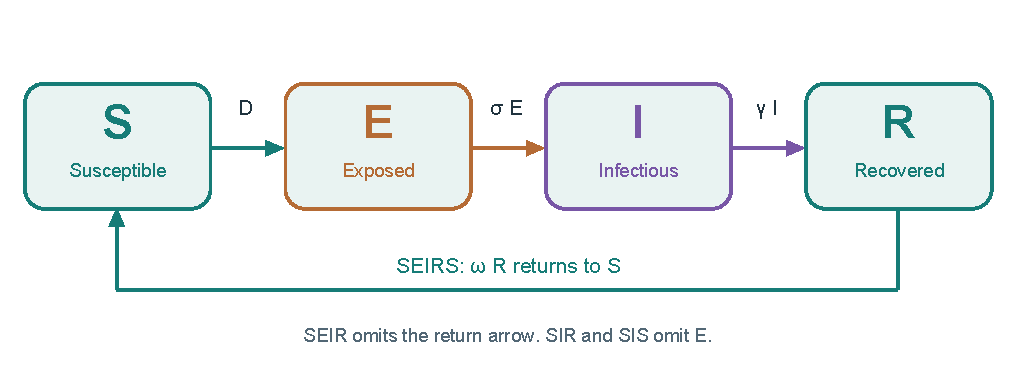
\includegraphics[width=1\linewidth,height=\textheight,keepaspectratio]{assets/simulation-guide/compartments.pdf}
\caption{Compartment transitions. Every arrow uses the state
at the start of the same day.}
\end{figure}

\subsection{Two transmission pathways}\label{two-transmission-pathways}

Contact transmission is an assumed process within a region. Movement
transmission depends on directed ledger records, including records whose
source and destination are the same region. Their contributions add to
the total hazard, so a local movement record and the contact term can
both contribute on the same day.

Trade changes exposure pressure while each region retains its population
\(N\). The recurrence tracks changes in compartment membership within
these fixed populations. This gives a compact representation of exposure
through movement; demographic processes and physical relocation would
require further state variables and balance equations.

\Needspace{14\baselineskip}
\subsection{Four model choices}\label{four-model-choices}

\begin{longtable}[]{@{}
  >{\raggedright\arraybackslash}p{(\linewidth - 4\tabcolsep) * \real{0.3333}}
  >{\raggedright\arraybackslash}p{(\linewidth - 4\tabcolsep) * \real{0.3333}}
  >{\raggedright\arraybackslash}p{(\linewidth - 4\tabcolsep) * \real{0.3333}}@{}}
\toprule\noalign{}
\begin{minipage}[b]{\linewidth}\raggedright
Model
\end{minipage} & \begin{minipage}[b]{\linewidth}\raggedright
Compartment path
\end{minipage} & \begin{minipage}[b]{\linewidth}\raggedright
Distinctive assumption
\end{minipage} \\
\midrule\noalign{}
\endhead
\bottomrule\noalign{}
\endlastfoot
SIR & S \ensuremath{\rightarrow} I \ensuremath{\rightarrow} R & No exposed stage; recovery removes susceptibility for
the run \\
SIS & S \ensuremath{\rightarrow} I \ensuremath{\rightarrow} S & Recovery immediately returns units to
susceptibility \\
SEIR & S \ensuremath{\rightarrow} E \ensuremath{\rightarrow} I \ensuremath{\rightarrow} R & A latent stage precedes infectiousness \\
SEIRS & S \ensuremath{\rightarrow} E \ensuremath{\rightarrow} I \ensuremath{\rightarrow} R \ensuremath{\rightarrow} S & Recovered units can lose protection \\
\end{longtable}

In SIR and SIS, new infection entries join \(I\) at the end of the day.
Their first contribution to transmission or recovery occurs in the
following daily transition. In SEIR and SEIRS, new entries join \(E\) at
the end of the day. Only the exposed units present at the day's start
can progress to \(I\) during it.

\subsection{Ledger mode and simulation
mode}\label{ledger-mode-and-simulation-mode}

Ledger mode describes allowed recorded movements and network statistics.
Simulation mode describes compartments and exposure calculations driven
by the canonical daily ledger. The two modes answer complementary
questions: Ledger mode describes the movement network, while Simulation
mode describes the model response to that network. Metric selection
changes the quantity displayed.

\section{Inputs and population
denominators}\label{inputs-and-population-denominators}

\subsection{The daily ledger}\label{the-daily-ledger}

Each usable record supplies a UTC calendar day, source region
\nolinkurl{COROP_LEV}, destination region \nolinkurl{COROP_AFN}, and
positive movement count \nolinkurl{AANTAL}. The engine combines records
sharing a day and directed route. \(A \to  B\) and \(B \to  A\) remain
different routes. \(A \to  A\) is a recorded local movement.

The engine requires a consecutive daily observation calendar. An
explicit calendar can include an empty movement day. The application
constructs its calendar from recorded dates and checks for gaps, so each
day needs a declared place in the input. Records with absent or
\texttt{NA} endpoints are excluded; a known but undeclared endpoint
raises an error. When preparing data, document both calendar coverage
and the completeness of the recorded movements.

\subsection{Synthetic population
construction}\label{synthetic-population-construction}

The default denominator is a constructed scale of model units. In the
available history before introduction, each region receives an activity
total equal to outgoing volume plus 0.7 times incoming volume. A local
record contributes to both parts. The history window is the 365 calendar
days before introduction; records on or after introduction do not
contribute.

\[
T_i=V^{out}_i+0.7V^{in}_i,\qquad z_i=\log(1+T_i)
\]

Let \(a\) and \(b\) be the smallest and largest positive \(z\) values.
For a region with positive activity and \(b > a\), the population
construction is:

\[
N_i=\mathrm{round}(450+9550(z_i-a)/(b-a))
\]

Zero activity receives 450 units. If the positive activities are all
equal, every region receives 450 units. The 0.7 weight, logarithm and
450--10,000 range are modelling choices. Together they define the scale
of the synthetic model population. The code stores this denominator in
the field \nolinkurl{holdings}; interpret its units through the
population metadata.

A prepared inventory can instead provide a fixed regional vector with a
declared reference, unit, date and geography. The inventory establishes
the denominator and its units; transmission coefficients remain separate
inputs. A region with \(N = 0\) has undefined prevalence. Positive
movement incident to such a region is rejected because the pressure
calculation requires a positive population denominator, including when a
scenario restricts that route.

\subsection{Initialization}\label{initialization}

With share initialization, initial percentages apply to the seed region
only. For \(N = 10{,}000\), an initial infectious share of 1\% supplies
\(I = 100\) in that region. The other regions begin susceptible. Exposed
and recovered percentages are separate inputs and the three percentages
must sum to at most 100.

Count initialization accepts explicit \(S/E/I/R\) values for every
region and requires initial percentages to be zero. This permits
multiple initially infected regions. Each explicit vector must conserve
its declared population. The tutorial script uses this form so that all
starting values are visible.

At the exact introduction boundary the engine records an
\nolinkurl{initialFrame}, then computes the day's transition. Before
introduction, compartments remain susceptible. Cumulative infection
entries begin at zero, with initial \(E\) and \(I\) recorded as starting
stocks. For a peak calculation, retain this initial boundary as well as
every daily end state.

Changing the introduction date can change more than timing. With
synthetic populations and share initialization it changes the historical
population calculation; it also changes the historical graph used by
several presets and the subsequent shipment calendar. For a timing
comparison, record which of these inputs are held fixed.

\section{The daily calculation}\label{the-daily-calculation}

\subsection{Step 1 Apply the day's
permissions}\label{step-1-apply-the-days-permissions}

Let \(x_{ij,t}\) be the recorded count on a route that remains allowed
after restrictions. A regional export restriction blocks routes from
that region to other regions. A regional import restriction blocks
routes from other regions into it. Neither closes its local route. A
dated route restriction blocks the specified route for that calendar
day, including a local route if explicitly selected.

All node changes dated on or before the day are applied before
calculating pressure. Node permissions persist until another event
changes them. Route restrictions are looked up for the current day only.
The default permission is allowed.

\subsection{Step 2 Compute movement
pressure}\label{step-2-compute-movement-pressure}

The source infectious share determines how much pressure a permitted
record supplies:

\[
L_{ij,t}=\kappa x_{ij,t}(I_{i,t}/N_i)
\]

\(\kappa \) is the Movement control. \(L\) has model population units
for that day's exposure calculation. It measures the exposure
contribution assigned to the route. All routes read the same start
state, so exposure acquired today can influence later daily
calculations.

\subsection{Step 3 Combine the pathways at each
recipient}\label{step-3-combine-the-pathways-at-each-recipient}

The contact hazard is proportional to the recipient's own infectious
share. Incoming movement pressure is divided by the recipient
population:

\[
h^c_{j,t}=\beta I_{j,t}/N_j
\]

\[
h^m_{j,t}=\sum_i L_{ij,t}/N_j,\qquad h_{j,t}=h^c_{j,t}+h^m_{j,t}
\]

The movement sum includes \(i = j\). For a fixed incoming pressure, a
larger recipient denominator gives a smaller hazard. At low hazard and a
fully susceptible destination, multiplying that hazard by the
susceptible population approximately cancels this denominator in the
incident count. The denominator still matters for fractions, depletion
and subsequent dynamics.

\subsection{Step 4 Convert hazard into new
entries}\label{step-4-convert-hazard-into-new-entries}

\[
p_{j,t}=1-\exp(-h_{j,t}),\qquad D_{j,t}=S_{j,t}p_{j,t}
\]

\(D\) is the number of new infection entries during the day. In SEIR it
enters \(E\). The exponential keeps the entry fraction between zero and
one for nonnegative finite hazard. At small hazard, \(D \approx  S h\);
at large hazard the susceptible stock limits entries.

The implementation uses \texttt{-Math.expm1(-h)} to evaluate
\(1 - \exp(-h)\) accurately when \(h\) is very small. The function
evaluates the exponential difference accurately near zero.

\begin{figure}
\centering
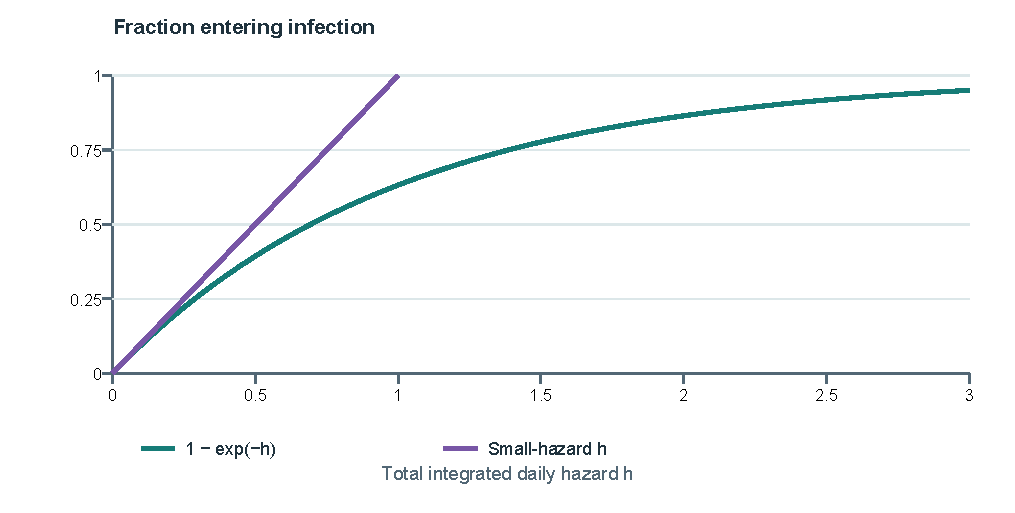
\includegraphics[width=1\linewidth,height=\textheight,keepaspectratio]{assets/simulation-guide/hazard.pdf}
\caption{The infection entry fraction and its linear
approximation at small hazard.}
\end{figure}

\subsection{Step 5 Advance compartments
simultaneously}\label{step-5-advance-compartments-simultaneously}

Define progression \(P = \sigma E\), recovery \(G = \gamma I\), and
immunity loss \(W = \omega R\) for SEIRS. SEIR sets \(W = 0\). Every
quantity on the right uses the start state:

\[
S_{t+1}=S_t-D_t+W_t,\qquad E_{t+1}=E_t+D_t-P_t
\]

\[
I_{t+1}=I_t+P_t-G_t,\qquad R_{t+1}=R_t+G_t-W_t
\]

For SIR, \(E = 0\), \(P = D\) and \(W = 0\). For SIS, \(E = R = 0\),
\(P = D\) and \(W = G\); the recovered amount goes directly back to
\(S\). To implement the update, calculate every flow from a copy of the
starting compartments, then write all four end states together. This
ordering gives each newly exposed unit its first opportunity to progress
during the following day.

\subsection{Step 6 Record states and
flows}\label{step-6-record-states-and-flows}

The engine records the end state, daily incident entries, cumulative
entries, movement pressure and route attribution. A frame's
\nolinkurl{date} or \nolinkurl{key} identifies the start of its
interval; \nolinkurl{intervalEnd} identifies when the stored compartment
state is observed. This distinction becomes essential when reading
weekly labels.

\subsection{Why the recurrence conserves
population}\label{why-the-recurrence-conserves-population}

Adding the four updates cancels \(D\), \(P\), \(G\) and \(W\). For valid
controls, \(0 \leq  D \leq  S\),
\(0 \leq  \sigma , \gamma , \omega  \leq  1\), and retained compartment
terms are nonnegative. Thus conservation and nonnegativity follow
directly from the equations. The engine checks these properties during
calculation.

The model is a discrete daily recurrence: the equations above define one
complete step. The exponential entry fraction treats the hazard as fixed
within that step. Progression, recovery and immunity loss use daily
fractions of the starting stocks. A continuous time model would instead
describe simultaneous change within the day through coupled differential
equations.

\clearpage
\section{Understanding the controls}\label{understanding-the-controls}

\begin{longtable}[]{@{}
  >{\raggedright\arraybackslash}p{(\linewidth - 4\tabcolsep) * \real{0.3333}}
  >{\raggedright\arraybackslash}p{(\linewidth - 4\tabcolsep) * \real{0.3333}}
  >{\raggedright\arraybackslash}p{(\linewidth - 4\tabcolsep) * \real{0.3333}}@{}}
\toprule\noalign{}
\begin{minipage}[b]{\linewidth}\raggedright
Control
\end{minipage} & \begin{minipage}[b]{\linewidth}\raggedright
Default
\end{minipage} & \begin{minipage}[b]{\linewidth}\raggedright
Meaning and units
\end{minipage} \\
\midrule\noalign{}
\endhead
\bottomrule\noalign{}
\endlastfoot
Model & SEIR & Selects the compartment recurrence \\
Seed region & CR35 & Region receiving the initial shares \\
Introduction & 1 Jan 2020 for the bundled calendar & Exact
initialization boundary \\
Initial infectious & 1\% of seed population & Starting infectious stock
as a share of the seed population \\
Initial exposed & 0\% & Starting exposed share in SEIR or SEIRS \\
Initial recovered & 0\% & Starting recovered share outside SIS \\
Contact \(\beta \) & 0.10 & Daily integrated contact hazard at unit
infectious share \\
Movement \(\kappa \) & 0.04 & Model units of pressure per recorded
animal at unit source infectious share \\
Progression \(\sigma \) & 0.22 & Daily fraction of starting \(E\)
entering \(I\) \\
Recovery \(\gamma \) & 0.15 & Daily fraction of starting \(I\) leaving
infectiousness \\
Immunity loss \(\omega \) & 0.02 & Daily fraction of starting \(R\)
returning to \(S\) in SEIRS \\
\end{longtable}

Contact and movement coefficients are finite, nonnegative quantities and
may exceed one. Progression, recovery and immunity loss are daily
fractions in \([0,1]\). Progression is active in SEIR and SEIRS;
immunity loss is active in SEIRS. Choose the model first, then interpret
the controls for the mechanisms it includes.

\subsection{Residence time is
geometric}\label{residence-time-is-geometric}

An isolated compartment with daily exit fraction \(q\) retains a
fraction \((1-q)^k\) after \(k\) transitions. For \(q > 0\), its mean
occupied grid time is \(1/q\) days. At the defaults, exposed and
infectious mean grid times are about 4.55 and 6.67 days; recovered
residence in SEIRS is 50 days. These means summarize a distribution of
residence times: part of a cohort exits early and part remains for
longer.

\[
\Pr(T=n)=(1-q)^{n-1}q,\qquad \mathrm{E}[T]=1/q
\]

At \(q = 0\), an isolated cohort never exits. At \(q = 1\), every member
present at the day's start exits during that transition. Newly arriving
members still wait until a later transition. For a continuous exit
hazard \(r\), matching one-day survival gives \(q = 1-\exp(-r)\).
Matching a desired geometric mean \(D\) gives \(q = 1/D\), when
\(D \geq  1\). Choose the conversion that matches the property being
specified: survival over a day or mean residence on the daily grid.

\begin{figure}
\centering
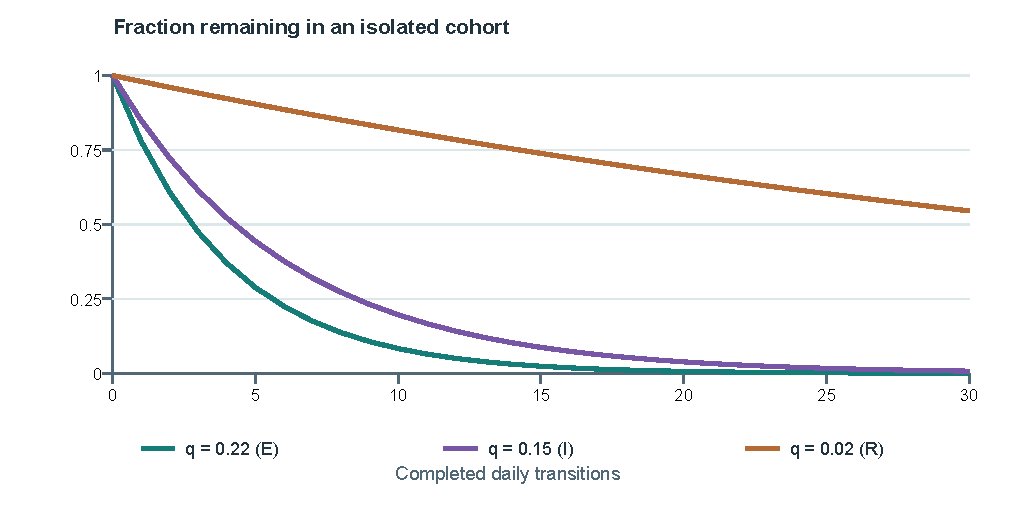
\includegraphics[width=1\linewidth,height=\textheight,keepaspectratio]{assets/simulation-guide/residence.pdf}
\caption{Surviving fractions under three daily exit fractions.
A long tail is part of the compartment assumption.}
\end{figure}

\subsection{What a parameter change can
influence}\label{what-a-parameter-change-can-influence}

Higher \(\beta \) increases the contact contribution at a fixed state.
Higher \(\kappa \) increases movement pressure at a fixed state. Over a
full trajectory, earlier growth can deplete susceptibles sooner and move
the peak forward. Compare the peak, its date and cumulative entries to
see these effects together.

Changing \(\sigma \) redistributes the timing of infectiousness.
Changing \(\gamma \) changes both the duration of infectiousness and how
much pressure can accumulate across days. Changing initial shares
changes the starting stock and its timing relative to shipments. These
mechanisms interact; a visually similar curve can arise from different
combinations. Interpreting a fitted curve therefore also requires
information about the quantities and processes used to estimate the
parameters.

\section{A complete two-region
example}\label{a-complete-two-region-example}

Consider fictional regions A and B, with populations 1,000 and 800 model
units. Start with the following counts. There is one permitted record of
80 animals from A to B and no other movement. Use the default SEIR
coefficients.

\begin{longtable}[]{@{}llllll@{}}
\toprule\noalign{}
Region & S & E & I & R & N \\
\midrule\noalign{}
\endhead
\bottomrule\noalign{}
\endlastfoot
A & 970 & 20 & 10 & 0 & 1,000 \\
B & 795 & 0 & 5 & 0 & 800 \\
\end{longtable}

\subsection{Pressure and incidence}\label{pressure-and-incidence}

A's infectious share is \(10/1000 = 0.01\). Its export pressure is
\(0.04 \times  80 \times  0.01 = 0.032\). B receives movement hazard
\(0.032/800 = 0.00004\). B's contact hazard is
\(0.10 \times  5/800 = 0.000625\), making total hazard \(0.000665\).

B's new entries are \(795 \times  [1-\exp(-0.000665)] = 0.528499\). A
has no incoming movements and produces
\(970 \times  [1-\exp(-0.001)] = 0.969515\) contact entries.

A progresses \(0.22 \times  20 = 4.4\) exposed units and recovers
\(0.15 \times  10 = 1.5\) infectious units. B has no exposed units to
progress and recovers \(0.15 \times  5 = 0.75\). The end state is:

\begin{longtable}[]{@{}llllll@{}}
\toprule\noalign{}
Region & S at end & E at end & I at end & R at end & New entries \\
\midrule\noalign{}
\endhead
\bottomrule\noalign{}
\endlastfoot
A & 969.030485 & 16.569515 & 12.900000 & 1.500000 & 0.969515 \\
B & 794.471501 & 0.528499 & 4.250000 & 0.750000 & 0.528499 \\
\end{longtable}

B's infectious count falls despite positive incidence, because incidence
enters \(E\) and recovery removes existing \(I\). A's infectious count
rises because its pre-existing exposed stock progresses. Both
populations remain exactly conserved up to floating-point precision. The
movement record contributes pressure while A's compartment total remains
1,000.

\subsection{Close A's exports at the start of this
day}\label{close-as-exports-at-the-start-of-this-day}

The A \ensuremath{\rightarrow} B route disappears from the exposure calculation. A's own update
is unchanged. B retains its contact hazard and produces
\(795 \times  [1-\exp(-0.000625)] = 0.496720\) entries. B still ends
with \(I = 4.25\) because its starting exposed stock and today's
recovery flow are the same in both runs. The difference first appears in
B's new exposed entries.

The one-day reduction in B's entries is about 0.031779. This is close
to, but not exactly equal to, the 0.031789 entries attributed to the
movement pathway in the open run. Attribution shares the total incident
count among simultaneous hazards; removal of a pathway recomputes the
nonlinear total. The two questions are distinct even in a single daily
step.

\Needspace{8\baselineskip}
\subsection{Run the example}\label{run-the-example}

From the repository root:

\begin{verbatim}
node scripts/simulation-tutorial-example.mjs
\end{verbatim}

The script imports the production engine, declares the fictional
population, runs the open and closed cases, and checks the hand
calculation, conservation and route attribution. It prints complete node
states and the route fields. Read \nolinkurl{initialStates},
\nolinkurl{nodeInterventions}, \nolinkurl{movementPressure},
\nolinkurl{newInfections} and \nolinkurl{riskLoad} together rather than
inspecting just the final curve.

\section{Reading pressure, incidence and
prevalence}\label{reading-pressure-incidence-and-prevalence}

\subsection{Movement pressure}\label{movement-pressure}

\(L_{ij}\) measures the route's assumed exposure pressure before
susceptible depletion and competing pathways. Regional incoming exposure
and outgoing pressure sum these quantities over routes between different
regions. They exclude local routes. Positive pressure can arrive at a
region with no susceptible units and cause zero incident entries.

\subsection{Infection entries and
attribution}\label{infection-entries-and-attribution}

The destination's total incident entries are \(D_{j}\). For a pathway
with hazard \(h_{k}\), the engine allocates:

\[
D_{k,j}=D_j h_{k,j}/h_j\quad \mathrm{when}\ h_j>0
\]

When total hazard is zero, all attributed entries are zero. The movement
route receives the share corresponding to its own movement hazard. The
local link collects contact attribution and attribution from any local
movement record. Therefore a local infection link can exist with zero
recorded local trade: it represents the separate contact contribution.

Link \nolinkurl{riskLoad} stores the attributed incident amount. Summing
link attribution into a destination recovers its total incident entries.
This accounting identity lets you connect each destination total to the
hazards that contributed to its calculation.

\subsection{Stocks, flows and cumulative
counts}\label{stocks-flows-and-cumulative-counts}

Prevalence is the infectious stock divided by population at an
observation time. Incidence is the flow of new entries during an
interval. Cumulative infections sum incident entries since
initialization and exclude the introduced \(E/I\) stock. In SIS and
SEIRS they count repeat entries, so they can exceed population. Their
unit follows the population definition used for the run.

National prevalence is \(\frac{\sum_i I_i}{\sum_i N_i}\), a population
weighted mean of regional infectious shares. A large region contributes
more weight. This distinction also explains why a striking regional peak
can coexist with a small national percentage.

\subsection{The pressure index}\label{the-pressure-index}

The internal field \nolinkurl{rtProxy} divides outgoing pressure by
infectious stock at the day's start. Over a displayed bin, it divides
summed outgoing pressure by summed daily start-state infectious stock,
recorded as \nolinkurl{infectiousUnitDays}. It is undefined when the
denominator is zero.

This measures outward movement pressure per infectious model unit per
day. A reproduction number answers a different question: how many
secondary infection entries arise over an infectious lifetime under
specified conditions. Deriving it requires population denominators,
transmission coefficients, compartment transitions and timing. Chapter
13 develops an example for a frozen movement matrix.

\section{Time labels and plotted
trajectories}\label{time-labels-and-plotted-trajectories}

\subsection{Three clocks}\label{three-clocks}

There is a \textbf{ledger day}, a \textbf{model transition}, and a
\textbf{display bin}. The first two are daily. The third may be daily,
weekly, monthly or yearly. Each display resolution summarizes the same
daily trajectory.

For a bin labelled 5 January covering
\([5 \text{January}, 12 \text{January})\), the displayed \(I\) is the
state after the 11 January transition, observed at the 12 January
boundary. New infections are summed over the seven daily intervals. A
closure on 8 January starts on 8 January inside this bin. Read the bin
label as its start date and the stored stock as its endpoint value.

\begin{figure}
\centering
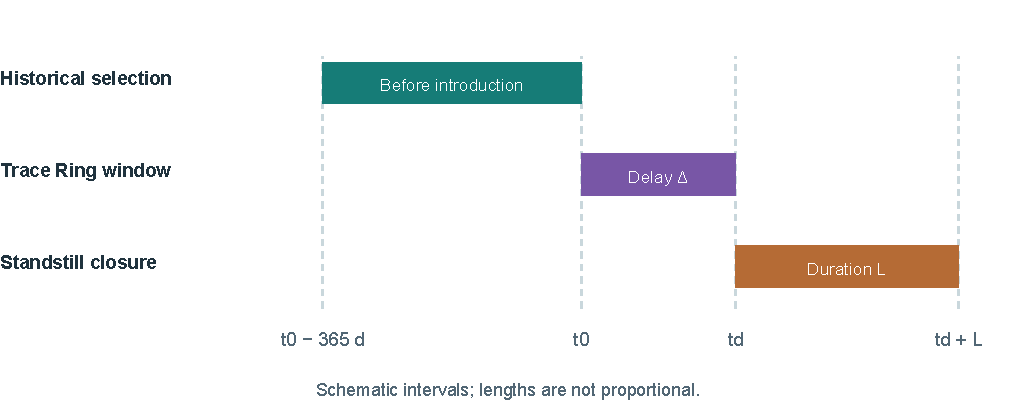
\includegraphics[width=1\linewidth,height=\textheight,keepaspectratio]{assets/simulation-guide/timing.pdf}
\caption{Historical selection, tracing, response and reopening
use distinct calendar intervals.}
\end{figure}

\begin{longtable}[]{@{}
  >{\raggedright\arraybackslash}p{(\linewidth - 2\tabcolsep) * \real{0.5000}}
  >{\raggedright\arraybackslash}p{(\linewidth - 2\tabcolsep) * \real{0.5000}}@{}}
\toprule\noalign{}
\begin{minipage}[b]{\linewidth}\raggedright
Quantity
\end{minipage} & \begin{minipage}[b]{\linewidth}\raggedright
Display aggregation
\end{minipage} \\
\midrule\noalign{}
\endhead
\bottomrule\noalign{}
\endlastfoot
S, E, I, R, prevalence & State at the actual end of the covered bin \\
New infections and attributed entries & Sum daily flows inside the
bin \\
Incoming exposure and outgoing pressure & Sum daily pressure inside the
bin \\
Cumulative infections & Cumulative value at the bin end \\
Population & The fixed vector or its total \\
Pressure index & Ratio of summed pressure to infectious unit-days \\
\end{longtable}

A partial final bin ends at the boundary of actual coverage. Summing a
week's starting infectious stocks, each weighted by one day, produces
infectious unit-days. Averaging daily prevalence gives mean prevalence
over the week. The chart instead displays prevalence at the bin
endpoint.

\subsection{Exact peaks and timeline
peaks}\label{exact-peaks-and-timeline-peaks}

The three-column panel's Timeline peak is the maximum of its displayed
trajectory. A weekly or monthly sample can miss the daily maximum. The
headless evaluator measures its peak over the introduction state and
daily end states. Use that daily path when reporting an exact maximum
and its date.

Chart interpolation is a drawing convention between available points.
The sampled values remain the observations used to draw the line. The
three-column view shares scales between corresponding figures, so a
visibly different height represents a numerical difference under that
shared metric. A figure in another region row can use a different scale;
the shared scale applies across the three columns for the same region.

\subsection{Choosing a resolution for Ledger
mode}\label{choosing-a-resolution-for-ledger-mode}

Coarse Ledger mode evaluates aggregated records at their date labels. It
can miss a closure inside a bin or apply start-date permissions to the
whole aggregate. Simulation mode applies daily restrictions before
computing its daily path. For exact retained-trade totals under dated
closures, use the daily ledger or the headless evaluator.

Selecting a date in the comparison overlay inspects stored values.
Editing a scenario setting changes its inputs and triggers a new
calculation after the 600 ms pause.

\section{The seven intervention
scenarios}\label{the-seven-intervention-scenarios}

An intervention has four parts: a target rule, a route action, a start
date, and a duration. A preset supplies those parts, while the
simulation controls supply the compartment model and coefficients.
Loading a preset in the single-scenario view replaces the existing
intervention schedule. The three-column view instead builds and
evaluates separate schedules without applying them to the live scenario.

Let introduction be \(t_0\), response delay be \(\Delta \), and response
be \(t_d = t_0 + \Delta \). Dates are calendar days. Standstill lasts
\(L\) days and applies on \([t_d, t_d+L)\): the opening boundary is
included and the reopening boundary is excluded. A response affects the
run from its start date through the remaining observation period.

\begin{longtable}[]{@{}
  >{\raggedright\arraybackslash}p{(\linewidth - 6\tabcolsep) * \real{0.2500}}
  >{\raggedright\arraybackslash}p{(\linewidth - 6\tabcolsep) * \real{0.2500}}
  >{\raggedright\arraybackslash}p{(\linewidth - 6\tabcolsep) * \real{0.2500}}
  >{\raggedright\arraybackslash}p{(\linewidth - 6\tabcolsep) * \real{0.2500}}@{}}
\toprule\noalign{}
\begin{minipage}[b]{\linewidth}\raggedright
Preset
\end{minipage} & \begin{minipage}[b]{\linewidth}\raggedright
Target rule
\end{minipage} & \begin{minipage}[b]{\linewidth}\raggedright
Action from response
\end{minipage} & \begin{minipage}[b]{\linewidth}\raggedright
What continues
\end{minipage} \\
\midrule\noalign{}
\endhead
\bottomrule\noalign{}
\endlastfoot
Open trade & No targets & Clear restrictions for the reference & All
movement and contact pathways \\
Seed containment & Seed region only & Close its exports to other regions
& Imports into seed, local movement and contact \\
Trace Ring & Seed plus its direct outgoing recipients during tracing &
Close each selected region's exports & Imports, local movement and
contact \\
Community Cordon & Seed's historical trade community & Close routes
leaving that community & Internal routes, incoming routes and contact \\
Hubs & Up to k historical outgoing-partner leaders & Close selected
regions' exports & Other exports, imports, local movement and contact \\
Bridges & Up to k historical betweenness leaders & Close selected
regions' exports & Other exports, imports, local movement and contact \\
Standstill & All regions & Close all routes between different regions
for L days & Local movement and contact; cross-region trade after
reopening \\
\end{longtable}

All persistent presets keep their target set fixed once constructed. The
intervention acts through movement permissions. Contact transmission and
compartment transitions continue under the selected simulation controls,
and each allowed movement follows its recorded route.

\subsection{Seed containment}\label{seed-containment}

This is an export action on the known seed. It removes later seed
exports from the pressure calculation. Imports into the seed, local
movements and contact transmission remain active. If recipients were
already exposed before response, they retain those compartments and
their own movement permissions. This is why a small delay can matter
even when the seed itself is controlled for the rest of the run.

\subsection{Trace Ring}\label{trace-ring}

The tracing window is \([t_0, t_d)\). The target set is the seed plus
every direct recipient of a positive seed export in that interval. The
window ends just before the response day. With zero delay, the window is
empty and only the seed is targeted.

Selection uses one step of outward movement from the seed. Each direct
recipient qualifies through a recorded export during the window,
regardless of its simulated infection count. Incoming partners and
further steps along the network lie outside this selection rule.

Longer response delays do two things together: they permit more days of
movement before closure and allow a larger tracing target set.
Consequently a Trace Ring delay comparison combines timing and scope.
The two mechanisms can act in opposing directions, producing a
nonmonotone sequence of outcomes.

\subsection{Historical selection for Cordon, Hubs and
Bridges}\label{historical-selection-for-cordon-hubs-and-bridges}

These strategies use positive routes between different regions in
\([t_0-365 \,\text{days}, t_0)\). Their application controls require a
full preceding year. The graph and its targets are anchored to the
history before introduction and remain fixed as response delay varies.

Repeated records on a route contribute to historical volume. Local
records are excluded from this targeting graph but remain part of the
simulation ledger and synthetic population calculation. Historical
topology, historical population construction and displayed network
statistics are three different uses of the data.

\subsection{Hubs}\label{hubs}

For each eligible source, count its distinct historical outgoing
destinations. Rank by that count, then outgoing volume, then region ID.
Choose the first \(k\), with at most the number of eligible regions. A
source with many small destinations can outrank one with a much larger
volume to a single destination. The ranking measures outward reach
through distinct destinations.

\subsection{Bridges}\label{bridges}

Construct a directed graph with an edge wherever historical volume is
positive. Compute node betweenness from shortest directed paths measured
in \textbf{hops}, giving equal shortest paths shared credit. Rank by
that score, then outgoing partner count, then region ID. Only regions
with at least one outgoing historical route are eligible; regions with
zero betweenness remain eligible when they meet that condition.

If \(n_{ab}\) counts shortest directed paths from a to b and
\(n_{ab}(v)\) counts those passing through v, the score is:

\[
B_v=\sum_{a,b} n_{ab}(v)/n_{ab}
\]

The sum excludes pairs where v is an endpoint and excludes equal
endpoints; an unreachable pair contributes zero. For the diamond A \ensuremath{\rightarrow} B \ensuremath{\rightarrow}
D and A \ensuremath{\rightarrow} C \ensuremath{\rightarrow} D, B and C each receive one half of the credit for the
pair A, D. Brandes' algorithm runs a breadth-first search from each
source to count shortest paths, then traverses the search order backward
to distribute dependency credit. It avoids enumerating every complete
path.

The Bridges selector uses directed, unweighted Brandes betweenness. The
Ledger panel uses weighted betweenness with inverse movement volume as
distance. Read each metric with its path length definition, since the
two definitions can produce different rankings. Brandes' publication
supplies background on the algorithm; the exact graph, eligibility and
tie rules are specified by HerdLink's selector code.
\href{https://doi.org/10.1080/0022250X.2001.9990249}{Brandes publication
record}.

\subsection{Community Cordon}\label{community-cordon}

For community selection, reciprocal historical volumes are combined into
an undirected weight. Louvain modularity optimization supplies the
partition. Broad uses resolution 1; Finer uses 1.5. The groups represent
trade connectivity. Louvain searches for a partition with high
modularity; its result can be a local optimum. Geographic adjacency
plays no role in that objective. A seed outside the historical graph
forms a singleton group.

If \(C_s\) is the seed community, the closure rule is
\(\mathrm{source} \in  C_s\) and \(\mathrm{destination} \notin  C_s\).
Movement in the opposite direction remains open. The implementation
applies this rule to recorded routes after response, including routes
that were absent from the historical graph. Community membership stays
fixed throughout the run.

The Louvain paper explains the general modularity method. HerdLink's
historical window, symmetrization and resolution values come from its
implementation. \href{https://arxiv.org/abs/0803.0476}{Blondel and
colleagues}. The displayed community panel describes a different graph
and period, so its membership need not match the targeting partition.

\subsection{Standstill}\label{standstill}

Standstill closes cross-region movement temporarily. Contact and
recorded local movement remain active, and existing \(E/I\) continue
through their compartment transitions. If those stocks survive until
reopening, movement can spread pressure again. A short pause can change
the time of a peak while changing the full-horizon cumulative count
little. Closing more routes for a shorter duration and closing fewer
routes persistently are different policy packages.

\section{Comparing scenarios in the
interface}\label{comparing-scenarios-in-the-interface}

Open Compare Scenarios with \texttt{C}, choose Simulation, and enable
Three scenarios. Each column can use a strategy or a saved scenario.
Preset columns use the active model settings and population; saved
scenarios retain their own saved settings and population. Shared axes
support visual comparison. To isolate an intervention effect, match the
other inputs using each column's settings information.

\begin{longtable}[]{@{}
  >{\raggedright\arraybackslash}p{(\linewidth - 4\tabcolsep) * \real{0.3333}}
  >{\raggedright\arraybackslash}p{(\linewidth - 4\tabcolsep) * \real{0.3333}}
  >{\raggedright\arraybackslash}p{(\linewidth - 4\tabcolsep) * \real{0.3333}}@{}}
\toprule\noalign{}
\begin{minipage}[b]{\linewidth}\raggedright
Recommended set
\end{minipage} & \begin{minipage}[b]{\linewidth}\raggedright
Columns
\end{minipage} & \begin{minipage}[b]{\linewidth}\raggedright
Factor intended to vary
\end{minipage} \\
\midrule\noalign{}
\endhead
\bottomrule\noalign{}
\endlastfoot
Strategies & Open trade, Seed containment, Trace Ring & Complete
intervention strategy \\
Target counts & Hubs with 1, 3 and 5 targets & Number of selected
regions \\
Response delays & Seed containment at 1, 7 and 14 days & Start of the
same target action \\
Pause duration & Standstill for 7, 14 and 28 days & Time until movement
reopens \\
\end{longtable}

Per-column inputs apply only where the strategy uses them. Target count
controls Hubs and Bridges; the Trace Ring and Cordon selection rules
determine their own group sizes. Pause duration controls Standstill.
Open trade has no response action. Editing a column waits 600 ms before
calculation; all three results are published together after they finish.
The comparison columns maintain their own evaluation schedules alongside
the live scenario.

The default region view shows three rows, selectable from one to five.
It ranks regions by the peak of the selected metric in the active
Original trajectory across the displayed timeline. All columns use these
same reference regions, making corresponding rows easy to compare.
Display sampling can influence the ranking because it determines the
points available for the peak calculation. Saved scenarios also use this
reference ranking.

\subsection{A comparison worksheet}\label{a-comparison-worksheet}

Before reading the curves, record the population reference and vector,
model, coefficients, initial state, seed, introduction, canonical
movement input and evaluation horizon. Then describe each schedule's
exact targets, route directions, start and end. Changes to any of these
inputs can contribute to a result difference.

For a simple timing lesson, set all columns to Seed containment with
delays 2, 3 and 7 days. Keep all other inputs matched. Inspect both
Prevalence and Cumulative infections. For a target-selection lesson,
compare Hubs and Bridges at equal \(k\), start date and duration,
alongside Open trade. Compare retained movement as well: regions
selected at equal target count can carry different amounts of trade.

Use a metric with a stated question. Peak infectious stock describes
maximum burden; its date describes timing. Cumulative entries describe
total model infection events over the horizon. Retained cross-region
movements describe disruption to this recorded ledger. A strategy can
improve one and worsen another. Interpret the trade-offs in relation to
the question posed by the comparison.

For exact retained trade, sum permitted daily movement counts over the
same post-introduction horizon and divide by the open reference's count.
If that denominator is zero, the ratio is undefined. Retained trade
measures the permitted share of the recorded ledger, with blocked
traffic removed and the other route counts held fixed.

\section{Understanding response
timing}\label{understanding-response-timing}

The bundled example introduces infection in CR35 on 1 January 2020.
There are no recorded exports from CR35 to other regions on that day. On
2 January, it exports to ten regions. A one-day response starts at the
beginning of 2 January and blocks those records. A two-day response
starts on 3 January and allows the first export day. The first export
day therefore creates a discrete change in which historical records
contribute pressure.

The parameter regime determines what happens after escape. Under a
hypothetical contact coefficient 0.32 and recovery fraction 0.15,
contact alone can amplify a small introduction in a largely susceptible
region. Once several regions have positive compartments, closing the
seed's later exports can leave a similar eventual susceptible depletion.
Peak timing may move even when final size changes little. Small
deterministic fractional stocks can persist through repeated daily
transitions.

The illustrative defaults use contact 0.10, movement 0.04, progression
0.22 and recovery 0.15. Contact alone is below its local growth
threshold. Recorded movements, including local records, can still
support growth. This setting illustrates how continued movement
contributes to the trajectory.

\begin{longtable}[]{@{}
  >{\raggedright\arraybackslash}p{(\linewidth - 4\tabcolsep) * \real{0.3333}}
  >{\raggedright\arraybackslash}p{(\linewidth - 4\tabcolsep) * \real{0.3333}}
  >{\raggedright\arraybackslash}p{(\linewidth - 4\tabcolsep) * \real{0.3333}}@{}}
\toprule\noalign{}
\begin{minipage}[b]{\linewidth}\raggedright
Seed response delay
\end{minipage} & \begin{minipage}[b]{\linewidth}\raggedright
Daily network prevalence peak
\end{minipage} & \begin{minipage}[b]{\linewidth}\raggedright
Cumulative infection entries
\end{minipage} \\
\midrule\noalign{}
\endhead
\bottomrule\noalign{}
\endlastfoot
1 day & 0.0428\% & 2,963 \\
2 days & 0.0496\% & 8,195 \\
3 days & 0.0555\% & 8,707 \\
7 days & 0.0680\% & 9,236 \\
\end{longtable}

These rounded values use the bundled daily ledger through its end, the
default synthetic population, CR35, introduction on 1 January 2020,
initial infectious share 1\%, SEIR, and persistent Seed containment.
Peaks include daily observations; cumulative entries exclude the
introduced seed. Counts are expressed in the synthetic population units
of the example. The two- and seven-day peaks differ by about 37\%, while
the cumulative totals differ by about 13\%.

Response effects follow the shipment calendar and the evolving
compartments. Weekend movement patterns, persistence of local
transmission, susceptible depletion, target changes in Trace Ring, and
Standstill reopening can all shape the result. Read both the size and
timing of peaks, and use a common horizon long enough to include the
features being compared.

\section{From code to a reproducible
result}\label{from-code-to-a-reproducible-result}

\subsection{The calculation chain}\label{the-calculation-chain}

The application reads and validates controls, obtains a population
snapshot, constructs dated restrictions, runs the shared daily engine,
aggregates daily output, and projects selected metrics into charts. The
unrestricted Original series reruns the same settings and daily input
with empty intervention schedules. It supplies the model reference
against which an intervention is compared.

\begin{itemize}
\tightlist
\item
  \textbf{Daily engine:} \nolinkurl{src/runtime/simulation-engine.js}.
  Start with \nolinkurl{validateSimulationSettings},
  \nolinkurl{prepareInputs}, \nolinkurl{simulateDaily} and
  \nolinkurl{aggregateDailyTrajectory} for validation, recurrence,
  accounting and aggregation.
\item
  \textbf{Population:} \nolinkurl{src/runtime/simulation-population.js}.
  Read \nolinkurl{estimateSyntheticPopulation},
  \nolinkurl{createSyntheticPopulationSnapshot} and
  \nolinkurl{validatePopulationSnapshot} for construction and metadata.
\item
  \textbf{Target selectors:}
  \nolinkurl{src/runtime/intervention-presets.js}. Read
  \nolinkurl{getHistoricalPresetGraph}, the target selectors and
  \nolinkurl{isCommunityCordonRoute} for historical graphs and selection
  rules.
\item
  \textbf{Application runtime:}
  \nolinkurl{src/runtime/herdlink-runtime.js}. Follow
  \nolinkurl{buildPresetScenario},
  \nolinkurl{buildSimulationTrajectory},
  \nolinkurl{evaluateComparisonScenario} and
  \nolinkurl{getOriginalSimulationSeries} from controls to calculated
  series.
\item
  \textbf{Comparison interface:}
  \nolinkurl{src/components/ScenarioComparison.jsx}. Follow the
  evaluation effect and metric projection for separate columns, delayed
  reruns and shared controls.
\item
  \textbf{Charts:} \nolinkurl{src/comparisonCharts.js}. Read
  \nolinkurl{pairComparisonSeries}, \nolinkurl{buildComparisonChart} and
  \nolinkurl{topComparisonRegions} for alignment, scales and ranking.
\item
  \textbf{Saved scenarios:} \nolinkurl{src/scenarioStorage.js}. Read the
  validation and serialization routines for the saved record format.
\end{itemize}

The application caches daily trajectories by a canonical identity
incorporating settings, population, dates, ledger and restriction
schedules. Display sampling summarizes the daily model. A cache hit
reuses a trajectory with the same complete input identity. Input
validation checks the controls and scenario records before calculation.

\subsection{Read a schedule as data}\label{read-a-schedule-as-data}

Node restrictions are a map from UTC midnight to a map of region
permissions. For example, one event closes A's exports and a later event
restores them. Each event changes its specified permission fields, so
imports and exports can be controlled independently.

\begin{verbatim}
new Map([
  [Date.parse("2020-01-08"), new Map([["A", { exports: false }]])],
  [Date.parse("2020-01-22"), new Map([["A", { exports: true }]])],
])
\end{verbatim}

This represents 14 restricted daily intervals. A route map keyed by 8
January and \texttt{A-B} represents a restriction on that route for that
day only. The application expands a route edit made in a coarse display
across the covered daily intervals. Read the resulting daily schedule to
identify the exact restricted intervals.

\subsection{Checking the calculation and assessing its
use}\label{checking-the-calculation-and-assessing-its-use}

Verification asks whether the program implements the declared equations.
Validation asks whether the model supports a particular empirical use.
The engine tests check fractional seeds, exact timing, state
conservation, directed pressure, synchronous updates, attribution,
undefined metrics and display invariance. These tests establish the
numerical and software properties used throughout the worked examples.
Empirical validation evaluates the relationship between model outputs
and observations for a stated application.

Run the following from the repository root:

\begin{verbatim}
node scripts/simulation-tutorial-example.mjs
node --test tests/simulation-engine.test.js tests/intervention-presets.test.js
node --test tests/evaluation-harness.test.js
\end{verbatim}

For the declared historical preset comparison, the evaluator imports the
same engine and target selectors, constructs schedules without browser
controls, and writes settings, metrics and input hashes:

\begin{verbatim}
node scripts/evaluate-scenario-presets.js reports/teaching-example --suite primary --seeds CR35 --scales broad
\end{verbatim}

The command writes the historical example as JSON and CSV, with separate
fields for daily peaks, infection entries and permitted trade. Preserve
the inputs and assumptions alongside any figure copied into a report.

\subsection{What to retain with a saved
result}\label{what-to-retain-with-a-saved-result}

Record engine identity, exact source version, coefficients, population
metadata and values, initialization convention and state, introduction,
daily data identity and coverage, restrictions, community scale, target
rule, display resolution, metric definition and horizon. Saved scenarios
use schema version 3 and \texttt{daily-contact-v1}. An inventory's
source date and geographic definition establish the reference for its
population counts.

When saved scenarios use different populations or model settings,
interpret their comparison as a difference between complete input
packages. For a comparison of interventions alone, match those inputs.
Private inventories remain in browser memory; public scenario slots
accept public population references.

\section{Mathematical interpretation and model
assumptions}\label{mathematical-interpretation-and-model-assumptions}

\subsection{Local growth near the susceptible
state}\label{local-growth-near-the-susceptible-state}

Consider one region, no recorded movement, \(S \approx  N\), and small
infectious amounts. Since \(1-\exp(-h) \approx  h\), new entries are
approximately \(\beta I\). In SIR, the early infectious update is:

\[
I_{t+1}\approx(1-\gamma+\beta)I_t
\]

Growth occurs when \(\beta  > \gamma \). In SEIR, the linearized updates
are:

\[
E_{t+1}\approx(1-\sigma)E_t+\beta I_t,\qquad I_{t+1}\approx\sigma E_t+(1-\gamma)I_t
\]

For positive progression and recovery, this two-compartment system
crosses its growth threshold at \(\beta  = \gamma \) as well.
Progression affects the time scale of growth. This argument assumes
near-complete susceptibility and removes all movement, including local
recorded movement. With movement present, add its pressure contribution
before interpreting growth.

\subsection{From a movement matrix to a transmission
matrix}\label{from-a-movement-matrix-to-a-transmission-matrix}

For a frozen allowed movement matrix and positive population vector,
linearization near susceptibility gives a transmission coefficient from
infectious units in source \(i\) to new entries in destination \(j\):

\[
C_{ji}=\beta\delta_{ji}+\kappa x_{ij}/N_i
\]

Here \(\delta \) is one when source and destination agree and zero
otherwise. Notice the source denominator after cancellation of the
susceptible recipient population. For constant common recovery
\(\gamma  > 0\), the expected number of occupied infectious grid
intervals is \(1/\gamma \). In this restricted frozen system, with
positive SEIR progression and no loss from the exposed stage, a
next-generation construction gives \(K = C/\gamma \) and threshold
\(\rho (K) = 1\).

This derivation uses a frozen movement matrix and nearly complete
susceptibility. In the daily model, shipments make the matrices time
dependent, their chronological product governs propagation, and
susceptible depletion changes the transmission process. The network
panel describes the movement matrix itself; the construction above also
incorporates transmission and recovery. General background on
next-generation constructions is given by
\href{https://pubmed.ncbi.nlm.nih.gov/19892718/}{Diekmann, Heesterbeek
and Roberts}; the derivation above states its own restricted
assumptions.

\subsection{Population and coefficient
interpretation}\label{population-and-coefficient-interpretation}

If every population and compartment amount is multiplied by a constant
\(c\) while ledger counts stay fixed, scaling \(\kappa \) by \(c\)
preserves prevalence trajectories under consistent initial shares.
Contact coefficients and daily exit fractions stay unchanged. This
transformation expresses the same prevalence dynamics in different model
count units. Changing the relative population sizes of regions changes
source shares and destination denominators by different factors, so it
alters the model beyond a common unit conversion.

\subsection{Relating model quantities to
observations}\label{relating-model-quantities-to-observations}

The ledger observes dated movements. Connecting it to compartments
requires further information about population sizes, infection states
and transitions. Several combinations of coefficients, initial states
and denominators can produce similar trajectories. Compartment counts,
test positivity, reported cases and farm outbreak status each need their
own relationship to the model state.

An empirical interpretation needs a stated unit and endpoint, population
measurements at that unit, dated observations with denominators, an
observation model, and evidence about reporting and diagnostic
processes. Parameter estimation and uncertainty assessment then need a
declared validation design. In a teaching exercise, settings can be
chosen to expose a mechanism clearly. In an empirical study, the
observation model and data determine how parameters are estimated and
assessed.

\subsection{The assumptions to carry into an
analysis}\label{the-assumptions-to-carry-into-an-analysis}

The model assumes complete mixing within each region, fixed populations,
constant coefficients, geometric exits, deterministic fractional states
and one daily ordering convention. Movement interventions act on
permissions while the contact coefficient remains fixed. Questions about
behaviour, rerouting, compliance, individual farms, shipment infection
status or demographic turnover would require those mechanisms to be
represented explicitly. Begin an analysis by deciding whether the stated
assumptions fit the question being studied.

\section{Exercises and worked
answers}\label{exercises-and-worked-answers}

Attempt the questions before reading the answers. Use the fictional
numbers to practise the equations and explain each result in words.

\subsection{Questions}\label{questions}

\textbf{1. Units.} A route carries 200 recorded animals, its source
infectious share is 0.02, and \(\kappa  = 0.04\). The destination has
population 1,000. Calculate route pressure and movement hazard. State
what each number measures.

\textbf{2. SEIR timing.} A region starts with \(E = 20\), \(I = 10\),
progression 0.22 and recovery 0.15. Today's new entries are 8. Calculate
its end-state \(E\) and \(I\). Identify which exposed stock supplies the
progression flow.

\textbf{3. Residence.} With recovery 0.15 and no new arrivals into
\(I\), what fraction of an infectious cohort remains after seven days?
What is its mean occupied grid time? Explain how these summaries
describe a distribution of residence times.

\textbf{4. Interval boundaries.} A Standstill starts on 8 January and
lasts 14 days. Is movement blocked on 21 January? On 22 January? How
many restricted daily intervals are there?

\textbf{5. Trace Ring.} The seed sends to B before introduction, C on
day 1 after introduction, D on day 2, and E on the day-3 response date.
F sends into the seed on day 1. Which regions are targeted for a
response delay of three days? Assume these are the only records.

\textbf{6. Cordon.} A community contains A and B. Which of A \ensuremath{\rightarrow} B, A \ensuremath{\rightarrow} C,
C \ensuremath{\rightarrow} A and A \ensuremath{\rightarrow} A is blocked by its cordon? What happens to A's contact
term?

\textbf{7. Aggregation.} A two-day bin has daily infection entries 2 and
3, infectious end states 10 and 12, and cumulative counts 7 and 10. What
are the bin's new infections, infectious stock and cumulative
infections?

\textbf{8. Attribution.} In the worked example, movement attribution is
0.031789 and the reduction after closing the route is 0.031779. Explain
why these two values differ.

\textbf{9. Population weighting.} Region A has population 100 and
infectious count 10; B has population 900 and infectious count 9.
Calculate national prevalence and the unweighted regional average. Which
does HerdLink display nationally?

\textbf{10. Targeting.} A has five outgoing historical partners and
volume 100; B has two partners and volume 10,000. Which wins the Hubs
ranking? Which additional outputs would you compare to assess model
burden and movement disruption?

\textbf{11. Local threshold.} With no recorded movements, near-full
susceptibility, \(\beta  = 0.10\) and \(\gamma  = 0.15\), calculate the
SIR early multiplier. Explain why a region with those controls might
still grow when movement is included.

\textbf{12. Comparison design.} Two saved scenarios differ in
population, contact coefficient and target count. Their shared-scale
plots differ. Explain what this comparison measures and describe a
second comparison that isolates target count.

\subsection{Worked answers}\label{worked-answers}

\textbf{1.} Pressure is \(0.04 \times  200 \times  0.02 = 0.16\) model
units for the day's calculation. Movement hazard is
\(0.16/1000 = 0.00016\). Pressure is the route contribution before
division by destination population; hazard enters the exponential
calculation. To obtain incident entries, combine all pathway hazards and
multiply the entry fraction by the susceptible stock.

\textbf{2.} Progression is \(0.22 \times  20 = 4.4\); recovery is
\(0.15 \times  10 = 1.5\). End-state \(E = 20 + 8 - 4.4 = 23.6\);
\(I = 10 + 4.4 - 1.5 = 12.9\). Progression uses the 20 exposed units
present at the start. The eight new entries become eligible to progress
during the next transition.

\textbf{3.} The remaining fraction is \(0.85^7 \approx  0.3206\), or
32.06\%. Mean occupied grid time is \(1/0.15 \approx  6.67\) days. Both
describe a distribution. Some of the cohort exits early and some remains
much longer.

\textbf{4.} Movement between different regions is blocked on 21 January
and allowed on 22 January. The restricted interval is
\([8 \text{January}, 22 \text{January})\), containing 14 daily steps.
Local movement and contact continue throughout.

\textbf{5.} The target set is the seed, C and D. B is before
introduction, E lies at the excluded response boundary, and F is an
incoming-only partner. Selection ends with these direct recipients of
the seed.

\textbf{6.} Only A \ensuremath{\rightarrow} C is blocked. Internal, inward and local routes
remain allowed. A's independent contact term remains active.

\textbf{7.} New infections are \(2 + 3 = 5\); the infectious stock is
12; cumulative infections are 10. Flows sum across the bin; stocks and
cumulative counts are read at its endpoint.

\textbf{8.} Attribution divides the incident count in one run among
simultaneous hazards. Closing a route changes the total hazard and
recomputes the exponential. The first value is a share within the open
run; the second is the difference between two runs. Nonlinearity makes
them slightly different.

\textbf{9.} National prevalence is \((10+9)/(100+900) = 1.9\%\). The
unweighted mean of 10\% and 1\% is 5.5\%. HerdLink displays the
population-weighted national share, 1.9\%.

\textbf{10.} A wins because Hubs first ranks distinct outgoing partners.
Volume breaks only a tie in partner count. Compare infection entries or
peak prevalence to assess model burden, and permitted movement totals to
assess disruption to the ledger. An economic cost calculation would also
need values assigned to that disruption.

\textbf{11.} The multiplier is \(1-0.15+0.10 = 0.95\). Contact alone
makes a small infectious stock decline in this approximation. Incoming
pressure and recorded local movement add to this contact contribution
and may change the direction of growth.

\textbf{12.} The first comparison measures the combined difference
between the two complete scenario packages. To isolate target count, run
both columns with the same population, coefficients, initial state,
ledger, dates and target rule, varying only the number of selected
regions. Shared scales then show the numerical difference for that
matched comparison.

\section{Reference sheet and sources}\label{reference-sheet-and-sources}

\subsection{Essential equations}\label{essential-equations}

\[
L_{ij}=\kappa x_{ij}I_i/N_i
\]

\[
h_j=\beta I_j/N_j+\sum_i L_{ij}/N_j,\qquad D_j=S_j[1-\exp(-h_j)]
\]

\[
P_j=\sigma E_j,\qquad G_j=\gamma I_j,\qquad W_j=\omega R_j\ \mathrm{in\ SEIRS}
\]

\[
S'=S-D+W,\quad E'=E+D-P,\quad I'=I+P-G,\quad R'=R+G-W
\]

Use start-state quantities on every right-hand side. For SEIR set
\(W = 0\); for SIR set \(E = 0, P = D, W = 0\); for SIS set
\(E = R = 0, P = D, W = G\). A restriction acts through the allowed
movement counts \(x\).

\subsection{Terms at a glance}\label{terms-at-a-glance}

\begin{longtable}[]{@{}
  >{\raggedright\arraybackslash}p{(\linewidth - 2\tabcolsep) * \real{0.5000}}
  >{\raggedright\arraybackslash}p{(\linewidth - 2\tabcolsep) * \real{0.5000}}@{}}
\toprule\noalign{}
\begin{minipage}[b]{\linewidth}\raggedright
Term
\end{minipage} & \begin{minipage}[b]{\linewidth}\raggedright
Meaning in this guide
\end{minipage} \\
\midrule\noalign{}
\endhead
\bottomrule\noalign{}
\endlastfoot
Stock & An amount at an observation time, such as I \\
Flow & An amount accumulated over an interval, such as new entries \\
Hazard & The integrated exposure quantity entering the exponential \\
Pressure & Movement count \ensuremath{\times} source infectious share \ensuremath{\times} movement
coefficient \\
Prevalence & Infectious stock divided by its population denominator \\
Counterfactual & A computed alternative under changed inputs within the
model \\
Attribution & Allocation of one run's incident entries among assumed
pathways \\
Verification & Checking implementation against its declared
specification \\
Validation & Assessing fitness for a stated empirical use \\
\end{longtable}

\subsection{Local sources}\label{local-sources}

The equations and application behaviour in this guide follow the source
tree inspected on 30 September 2026, using engine identity
\texttt{daily-contact-v1}. The following files connect each topic to its
implementation and tests.

\begin{itemize}
\tightlist
\item
  \href{../../src/runtime/simulation-engine.js}{Daily engine} and
  \href{../../tests/simulation-engine.test.js}{engine tests}: recurrence,
  units, timing, accounting and aggregation.
\item
  \href{../../src/runtime/simulation-population.js}{Population module} and
  \href{../../docs/simulation-population.md}{population notes}: denominator
  construction and reference handling.
\item
  \href{../../src/runtime/intervention-presets.js}{Preset selectors} and
  \href{../../docs/network-scenarios.md}{scenario specification}: target rules,
  observation windows and actions.
\item
  \href{../../src/runtime/herdlink-runtime.js}{Application runtime} and
  \href{../../src/components/ScenarioComparison.jsx}{three-column
  component}: control wiring, separate evaluations, timing and chart
  inputs.
\item
  \href{../../docs/simulation-model.md}{Model specification} and
  \href{../../docs/simulation-scientific-assessment.md}{scientific assessment}:
  mathematical contract and scope of interpretation.
\item
  \href{../../scripts/simulation-tutorial-example.mjs}{Tutorial example}:
  the fictional calculation in Chapter 6, with executable checks.
\item
  \href{../../scripts/evaluate-scenario-presets.js}{Evaluation harness} and
  \href{../../tests/evaluation-harness.test.js}{harness test}: historical
  example, reproducibility fields and checks on illustrative response
  separation.
\end{itemize}

\subsection{Further reading}\label{further-reading}

\textbf{Brandes, U. (2001).} A faster algorithm for betweenness
centrality. \emph{Journal of Mathematical Sociology}, 25(2), 163--177.
\href{https://doi.org/10.1080/0022250X.2001.9990249}{DOI and publication
record}. Read for shortest-path dependency accumulation; HerdLink's
exact targeting choices are documented in its source.

\textbf{Blondel, V. D., Guillaume, J.-L., Lambiotte, R., and Lefebvre,
E. (2008).} Fast unfolding of communities in large networks.
\emph{Journal of Statistical Mechanics}, P10008.
\href{https://arxiv.org/abs/0803.0476}{Author manuscript}. Read for the
modularity optimization underlying Louvain; Chapter 9 connects that
method to HerdLink's historical window and cordon action.

\textbf{Diekmann, O., Heesterbeek, J. A. P., and Roberts, M. G. (2010).}
The construction of next-generation matrices for compartmental epidemic
models. \emph{Journal of the Royal Society Interface}, 7(47), 873--885.
\href{https://pubmed.ncbi.nlm.nih.gov/19892718/}{Publication and
abstract}. Read for the distinction between a transmission model's
next-generation construction and a raw adjacency matrix. Chapter 13
derives a frozen matrix example from HerdLink's recurrence.
\end{document}
